%
%% Please do not remove author note!
%%%
%%%% Created by Kacper B Sokol (k.sokol.2011 [at] my.bristol.ac.uk)
%%%
%% Please do not remove author note!
%

\documentclass{beamer}


\usepackage{lipsum}

\usepackage{color}
\definecolor{CERNish}{RGB}{000,083,161}
\definecolor{CERNish-sup}{RGB}{192,192,192}

\setbeamercolor{structure}{fg=CERNish, bg=CERNish-sup}

% Slides background
\usepackage{tikz}								 % opaque logo in the background
\usebackgroundtemplate{
	\tikz\node[opacity=0.25]{
		\noindent \hspace{-12.2mm} \vspace{-0.3mm} \includegraphics*[width=1.2\paperwidth]{./gfx/bg.png}
		% ,height=\paperheight
	};
}

% Title page logo
\titlegraphic{
	% \vspace*{1cm}
	\mbox{ \hspace{0.697916667cm} 
\includegraphics[height=2cm]{./gfx/LogoOutline-Blue.png} \hspace{0.697916667cm} }
	% \hspace*{4.75cm}~
	\hspace*{3.25cm}~
	% space is 1.697916667 * image height i.e. (1.697916667*2cm -2cm) = (3.395833334cm -2cm)/2 = 0.697916667
	
\includegraphics[height=2cm]{./gfx/openlab-transparent.png}
	% collaboration logo
	\vspace*{0.3cm}
	
\includegraphics[height=.7cm]{./gfx/siemens-transparent.png}
}

\setbeamertemplate{navigation symbols}{}
\usepackage{beamerthemeshadow}

\expandafter\def\expandafter\insertshorttitle\expandafter{%
  \insertshorttitle\hfill%
  \insertframenumber}

% References
% \usepackage{biblatex}
% \addbibresource{bibliography.bib}

%%%%%%%%%%%%%%%%%%%%%%%%%%%%%%%%%%%%%%%%%%%%%%%%%%%%%%%%%%%%%%%%%%%%%%%%%%%%%%%%
%%%%%%%%%%%%%%%%%%%%%%%%%%%%%%%%%%%%%%%%%%%%%%%%%%%%%%%%%%%%%%%%%%%%%%%%%%%%%%%%
%%%%%%%%%%%%%%%%%%%%%%%%%%%%%%%%%%%%%%%%%%%%%%%%%%%%%%%%%%%%%%%%%%%%%%%%%%%%%%%%
%%%%%%%%%%%%%%%%%%%%%%%%%%%%%%%%%%%%%%%%%%%%%%%%%%%%%%%%%%%%%%%%%%%%%%%%%%%%%%%%
%%%%%%%%%%%%%%%%%%%%%%%%%%%%%%%%%%%%%%%%%%%%%%%%%%%%%%%%%%%%%%%%%%%%%%%%%%%%%%%%
%%%%%%%%%%%%%%%%%%%%%%%%%%%%%%%%%%%%%%%%%%%%%%%%%%%%%%%%%%%%%%%%%%%%%%%%%%%%%%%%
\usepackage{listings}
\definecolor{navyb}{RGB}{0100,043,054}
\lstset{
  captionpos=b,
  frame=single,
  emph={module, import, create, schema, as, @Name, @Description, select, from, win:time},
  emphstyle={\color{navyb}\bfseries},
}

\makeatletter
\define@key{beamerframe}{foot}[true]{
  \setbeamertemplate*{footline}
  \setbeamertemplate{headline}[default]
  \def\beamer@entrycode{\vspace*{-\headheight}}
}
\makeatother

\newenvironment{foot}{
  \setbeamertemplate*{footline}
  \makeatletter
    \setbeamertemplate{headline}[default]
    \def\beamer@entrycode{\vspace*{-\headheight}}
  \makeatother
}

\begin{document}

\title{Making sense of data streams}
\subtitle{Complex Event Processing for Controls Applications}
\author{Kacper B. Sokol}
\institute{CERN, EN/ICE}
\date{\today}

\begin{frame}[plain]
	\titlepage
\end{frame}

% \begin{frame}[foot]
%   \frametitle{Table of contents}
%   \tableofcontents
% \end{frame}

%%%% CONTENT %%%%

\section{Background} 
  \subsection{Signals}
  \begin{frame}[foot]
    \frametitle{Dynamic vs.\ Static}
    \begin{figure}
      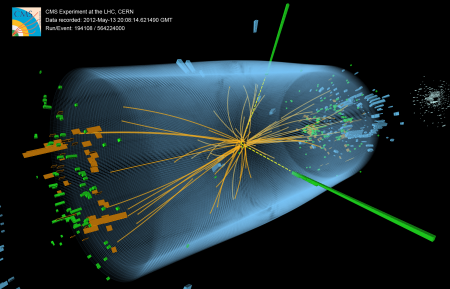
\includegraphics[scale=.7]{./gfx/CMS.png}
    \end{figure}
  \end{frame}

  \begin{frame}[foot]
    \frametitle{Data Points}
    \begin{figure}
      \includegraphics[scale=.42]{./gfx/f5f6.png}
    \end{figure}
  \end{frame}

  \begin{frame}[foot]
    \frametitle{Data Points in time}
    \begin{figure}
      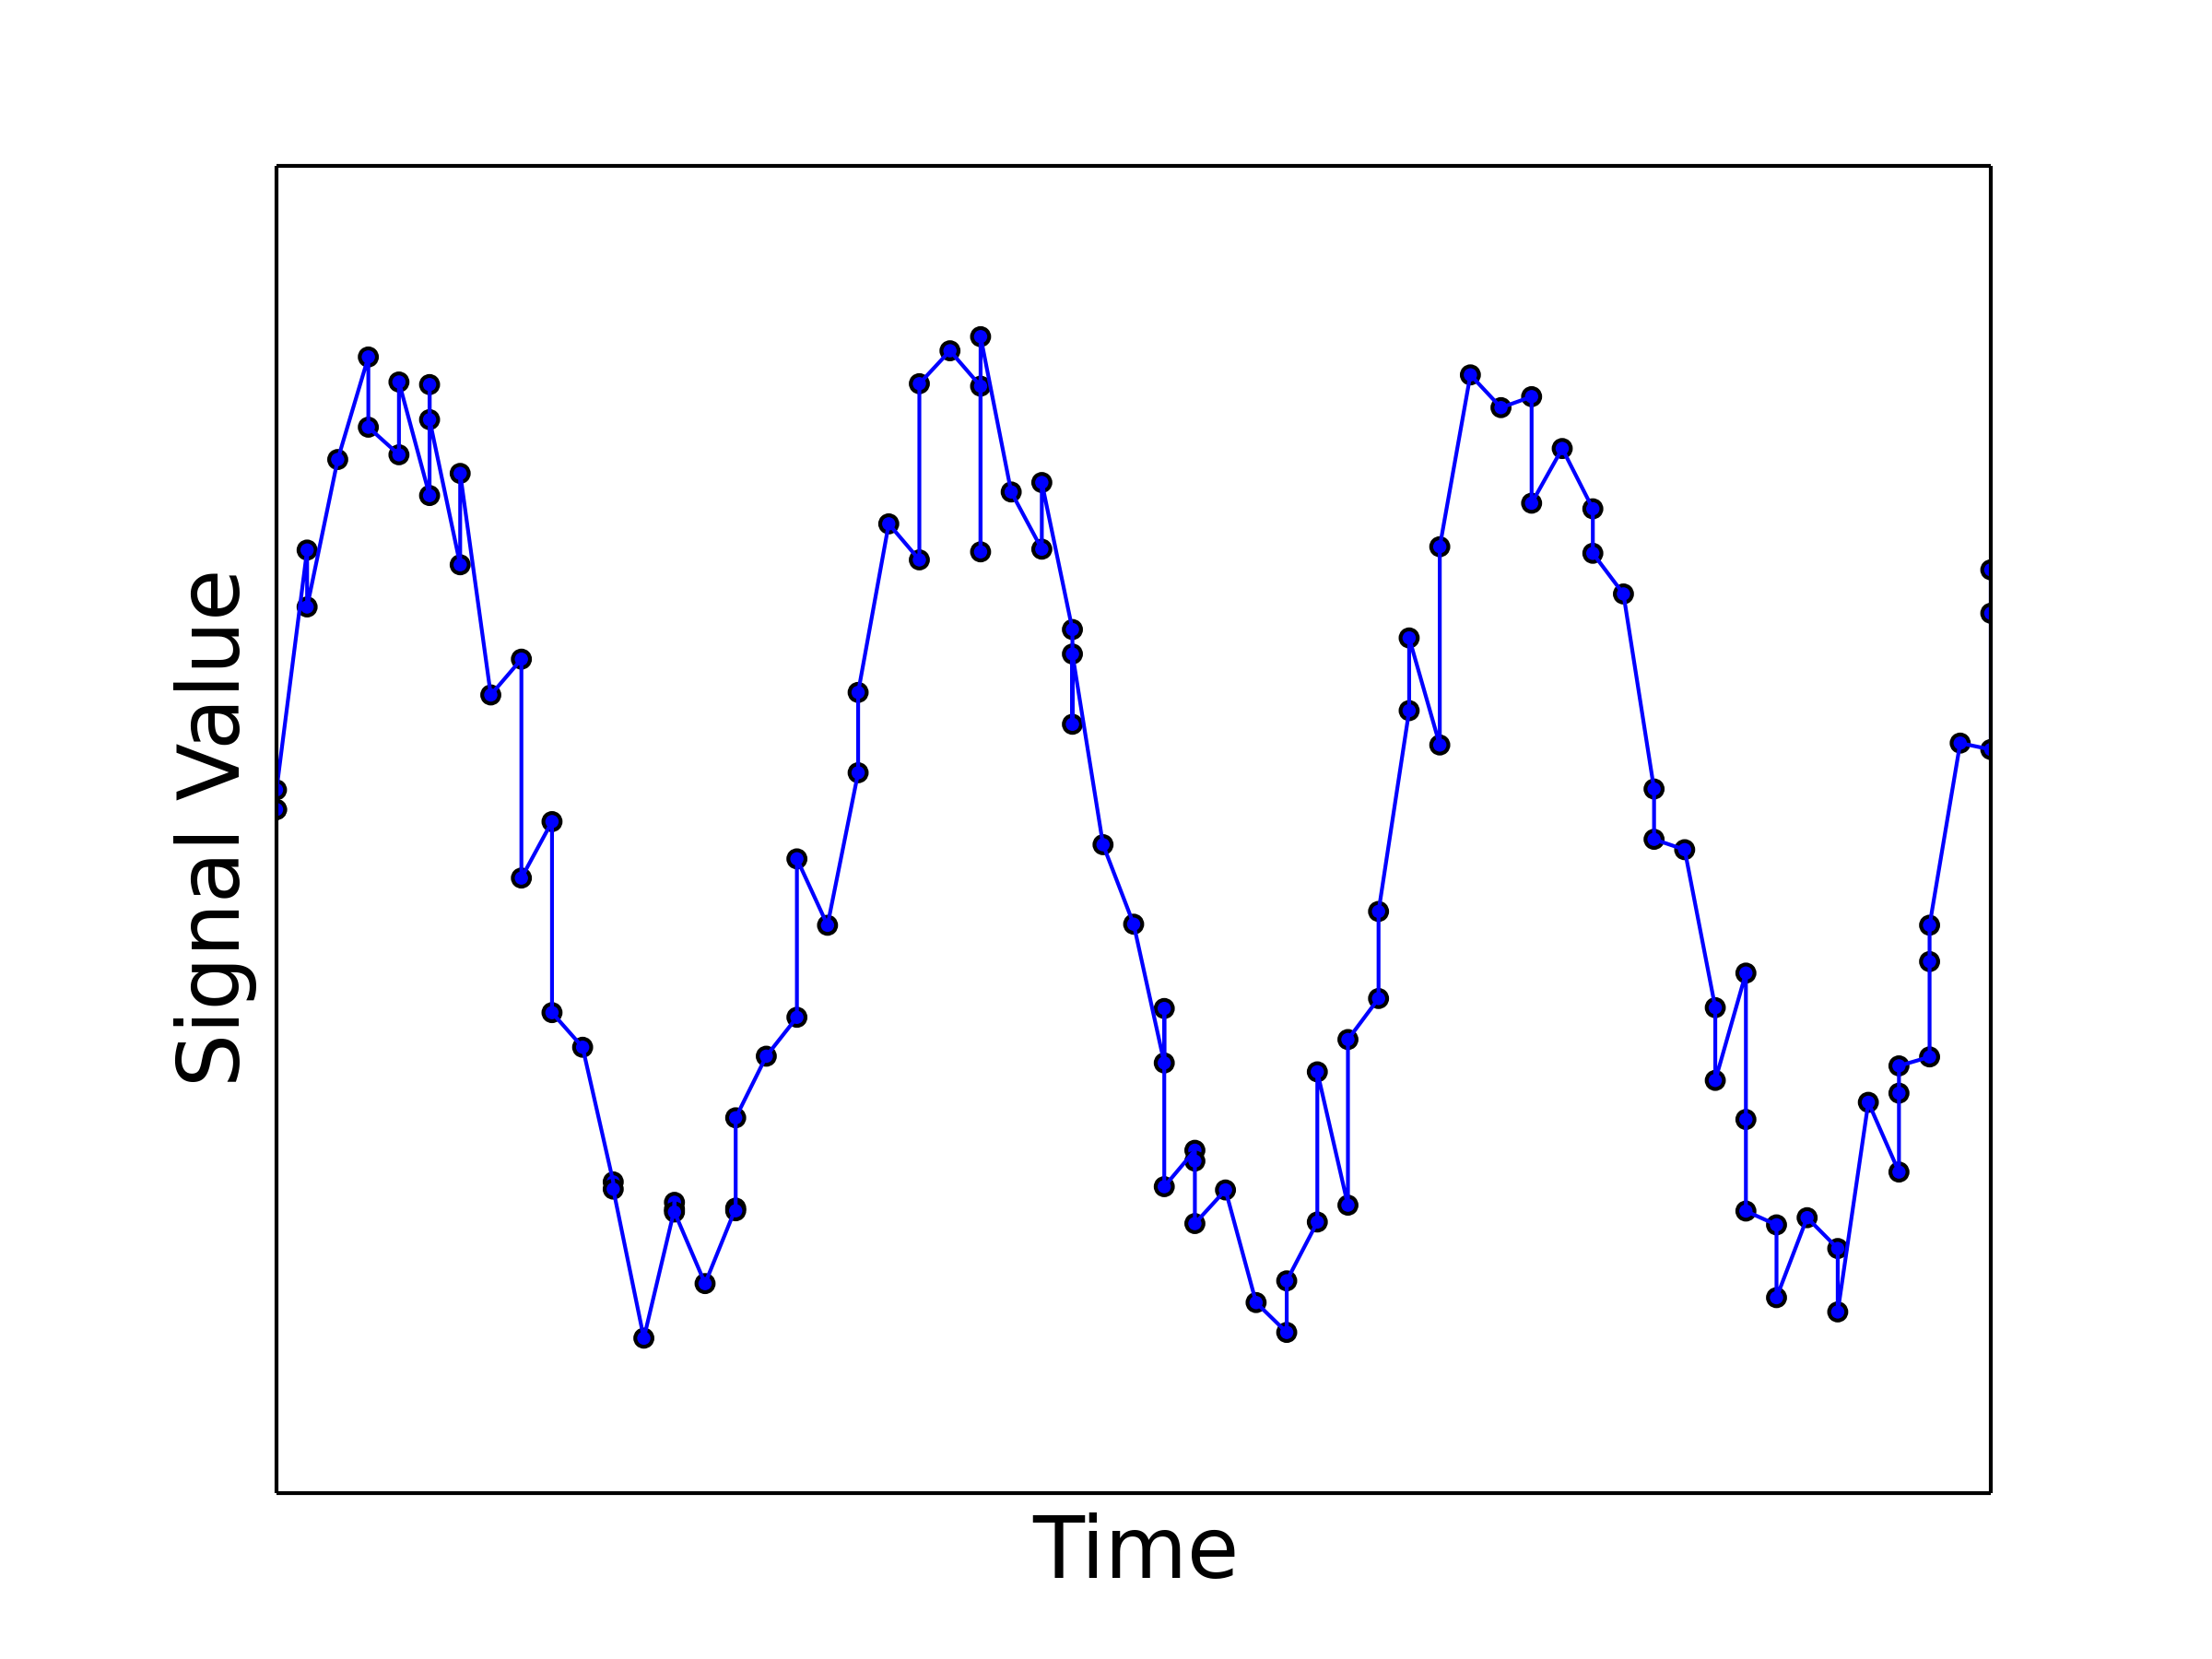
\includegraphics[scale=.5]{./gfx/feature5.png}
    \end{figure}
  \end{frame}

  \subsection{Signals Statistics}
  \begin{frame}[foot]
    \frametitle{Basic measures}
    \begin{block}{Time Windowing}
      \begin{itemize}
        \item Length;
        \item Time Window;
        \item Time Batch.
      \end{itemize}
    \end{block}
    \begin{block}{Measures}
      \begin{itemize}
        \item Average;
        \item Standard Deviation;
        \item $k$-Lag;
        \item etc.\
      \end{itemize}
    \end{block}
  \end{frame}

  \begin{frame}[foot]
    \frametitle{\texttt{avg}}
    \begin{figure}
      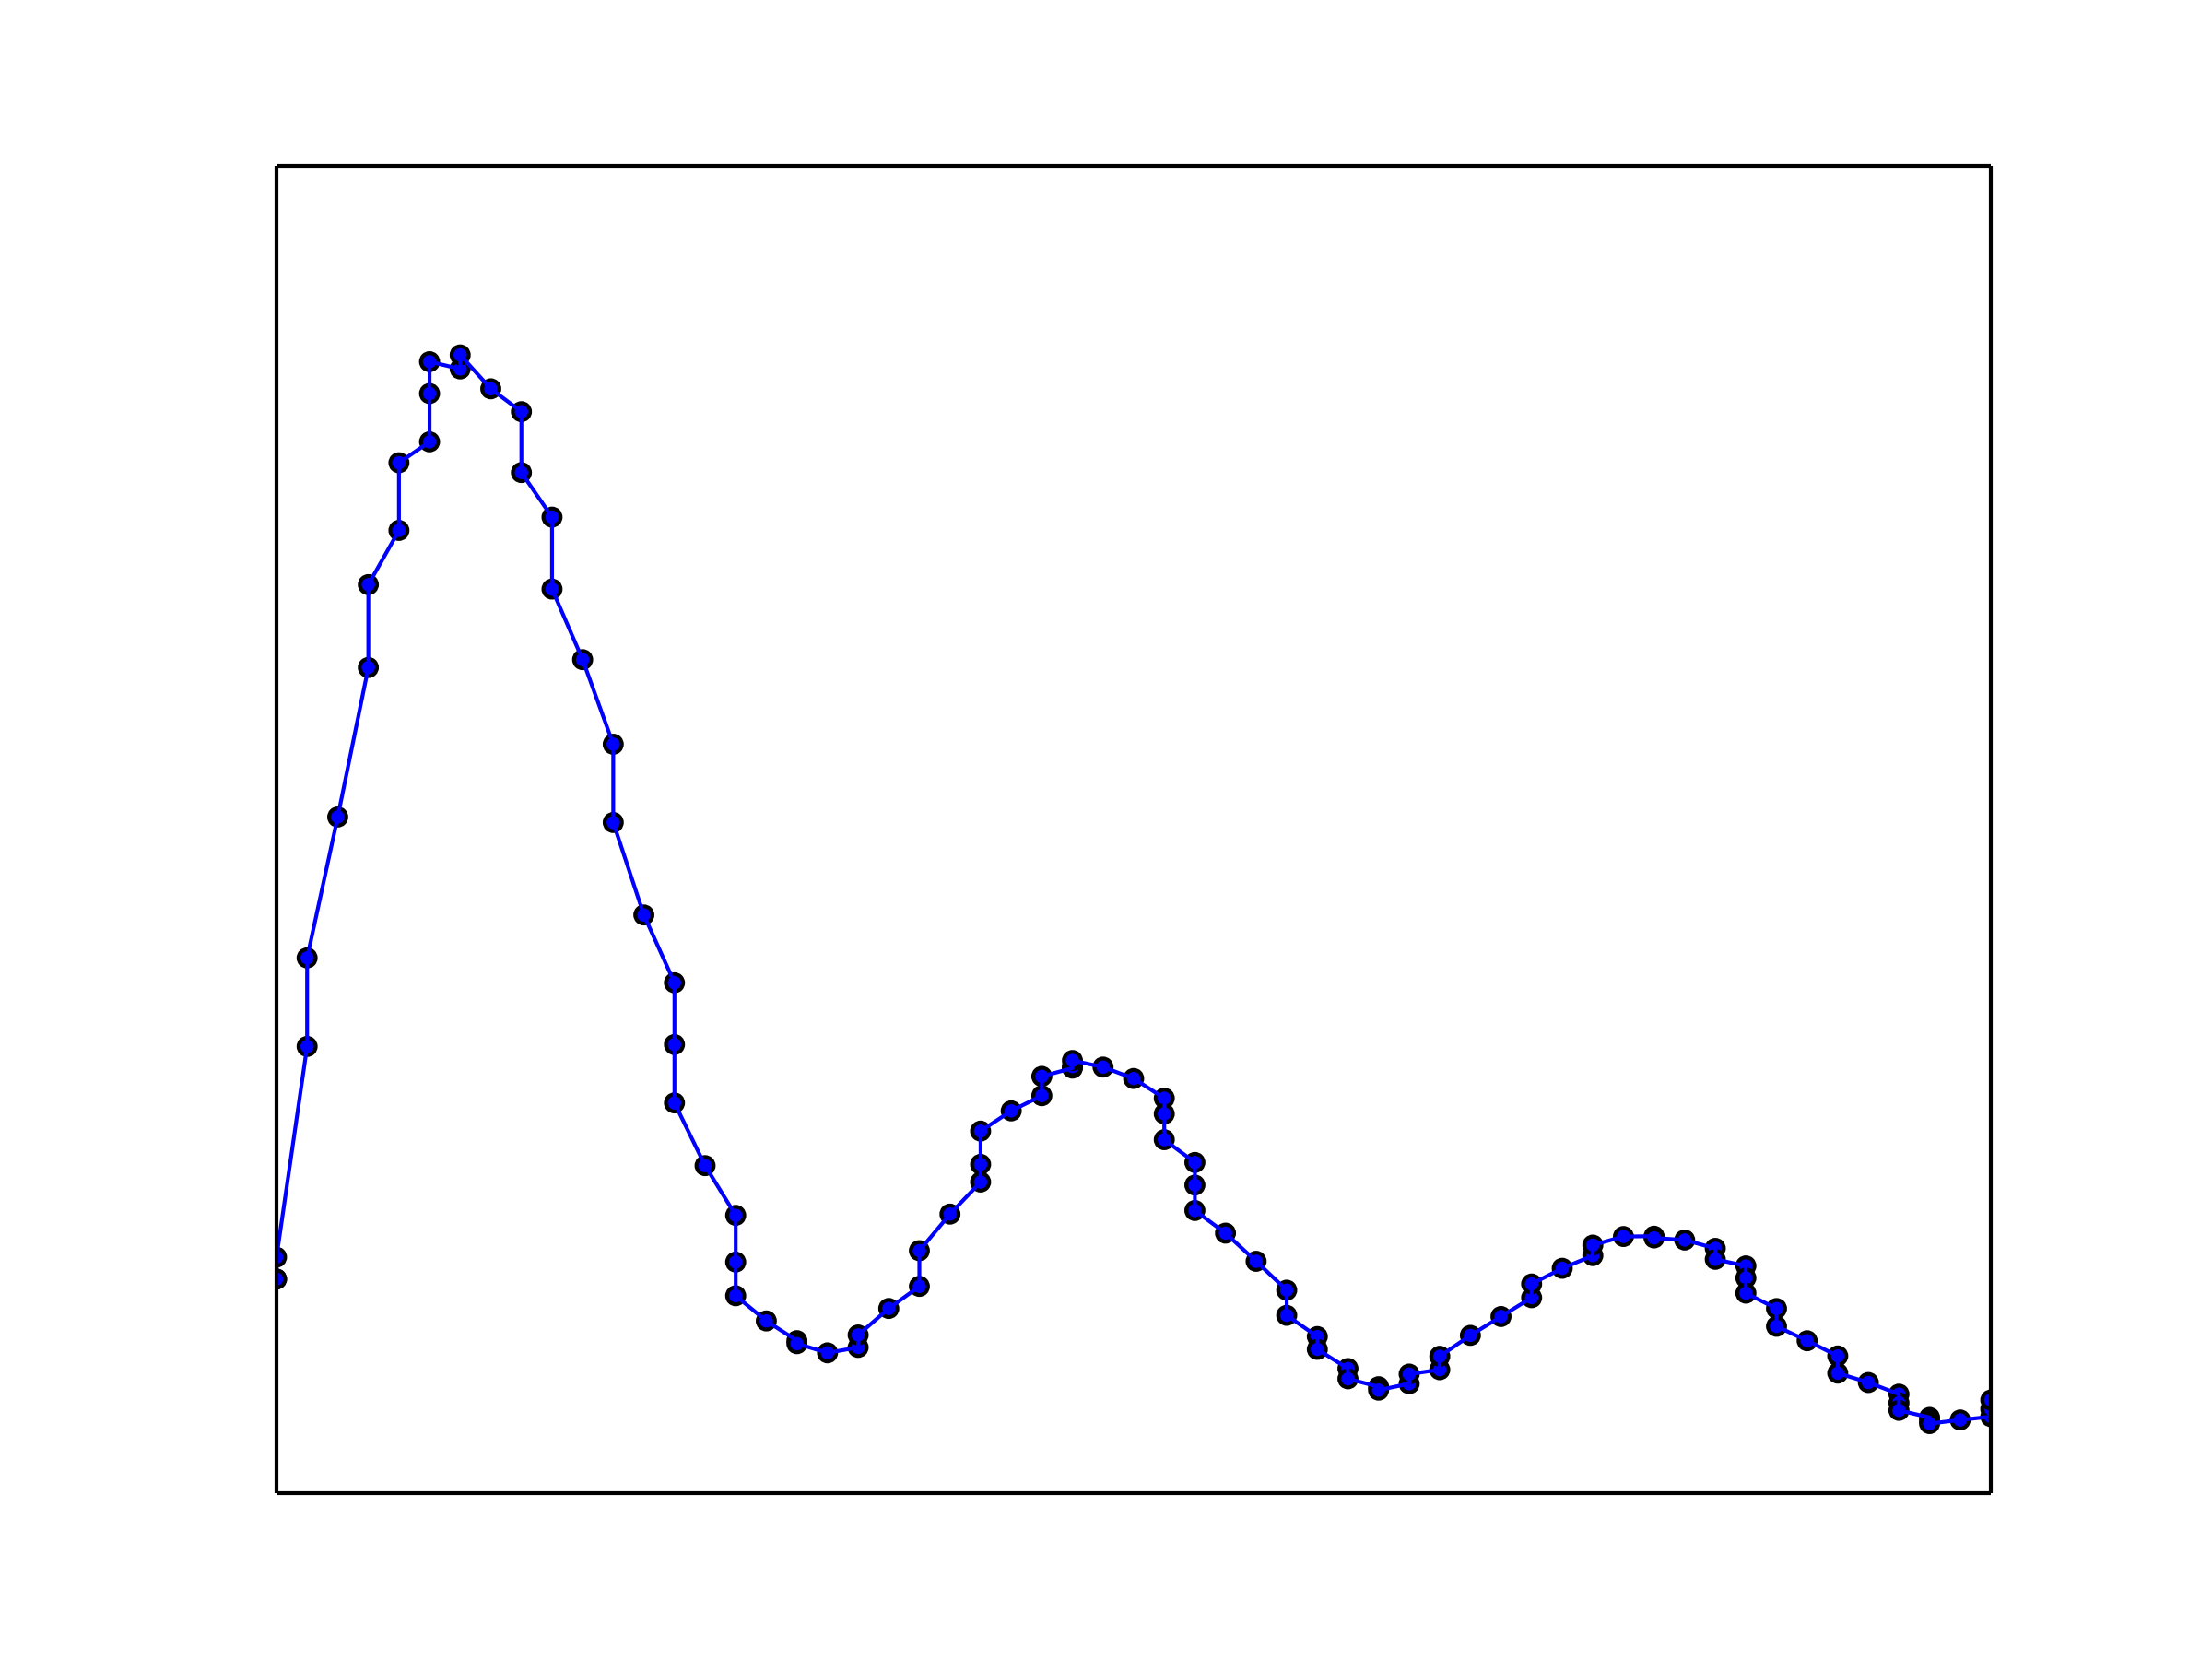
\includegraphics[scale=.5]{./gfx/feature1.png}
    \end{figure}
  \end{frame}

  \begin{frame}[foot]
    \frametitle{\texttt{std}}
    \begin{figure}
      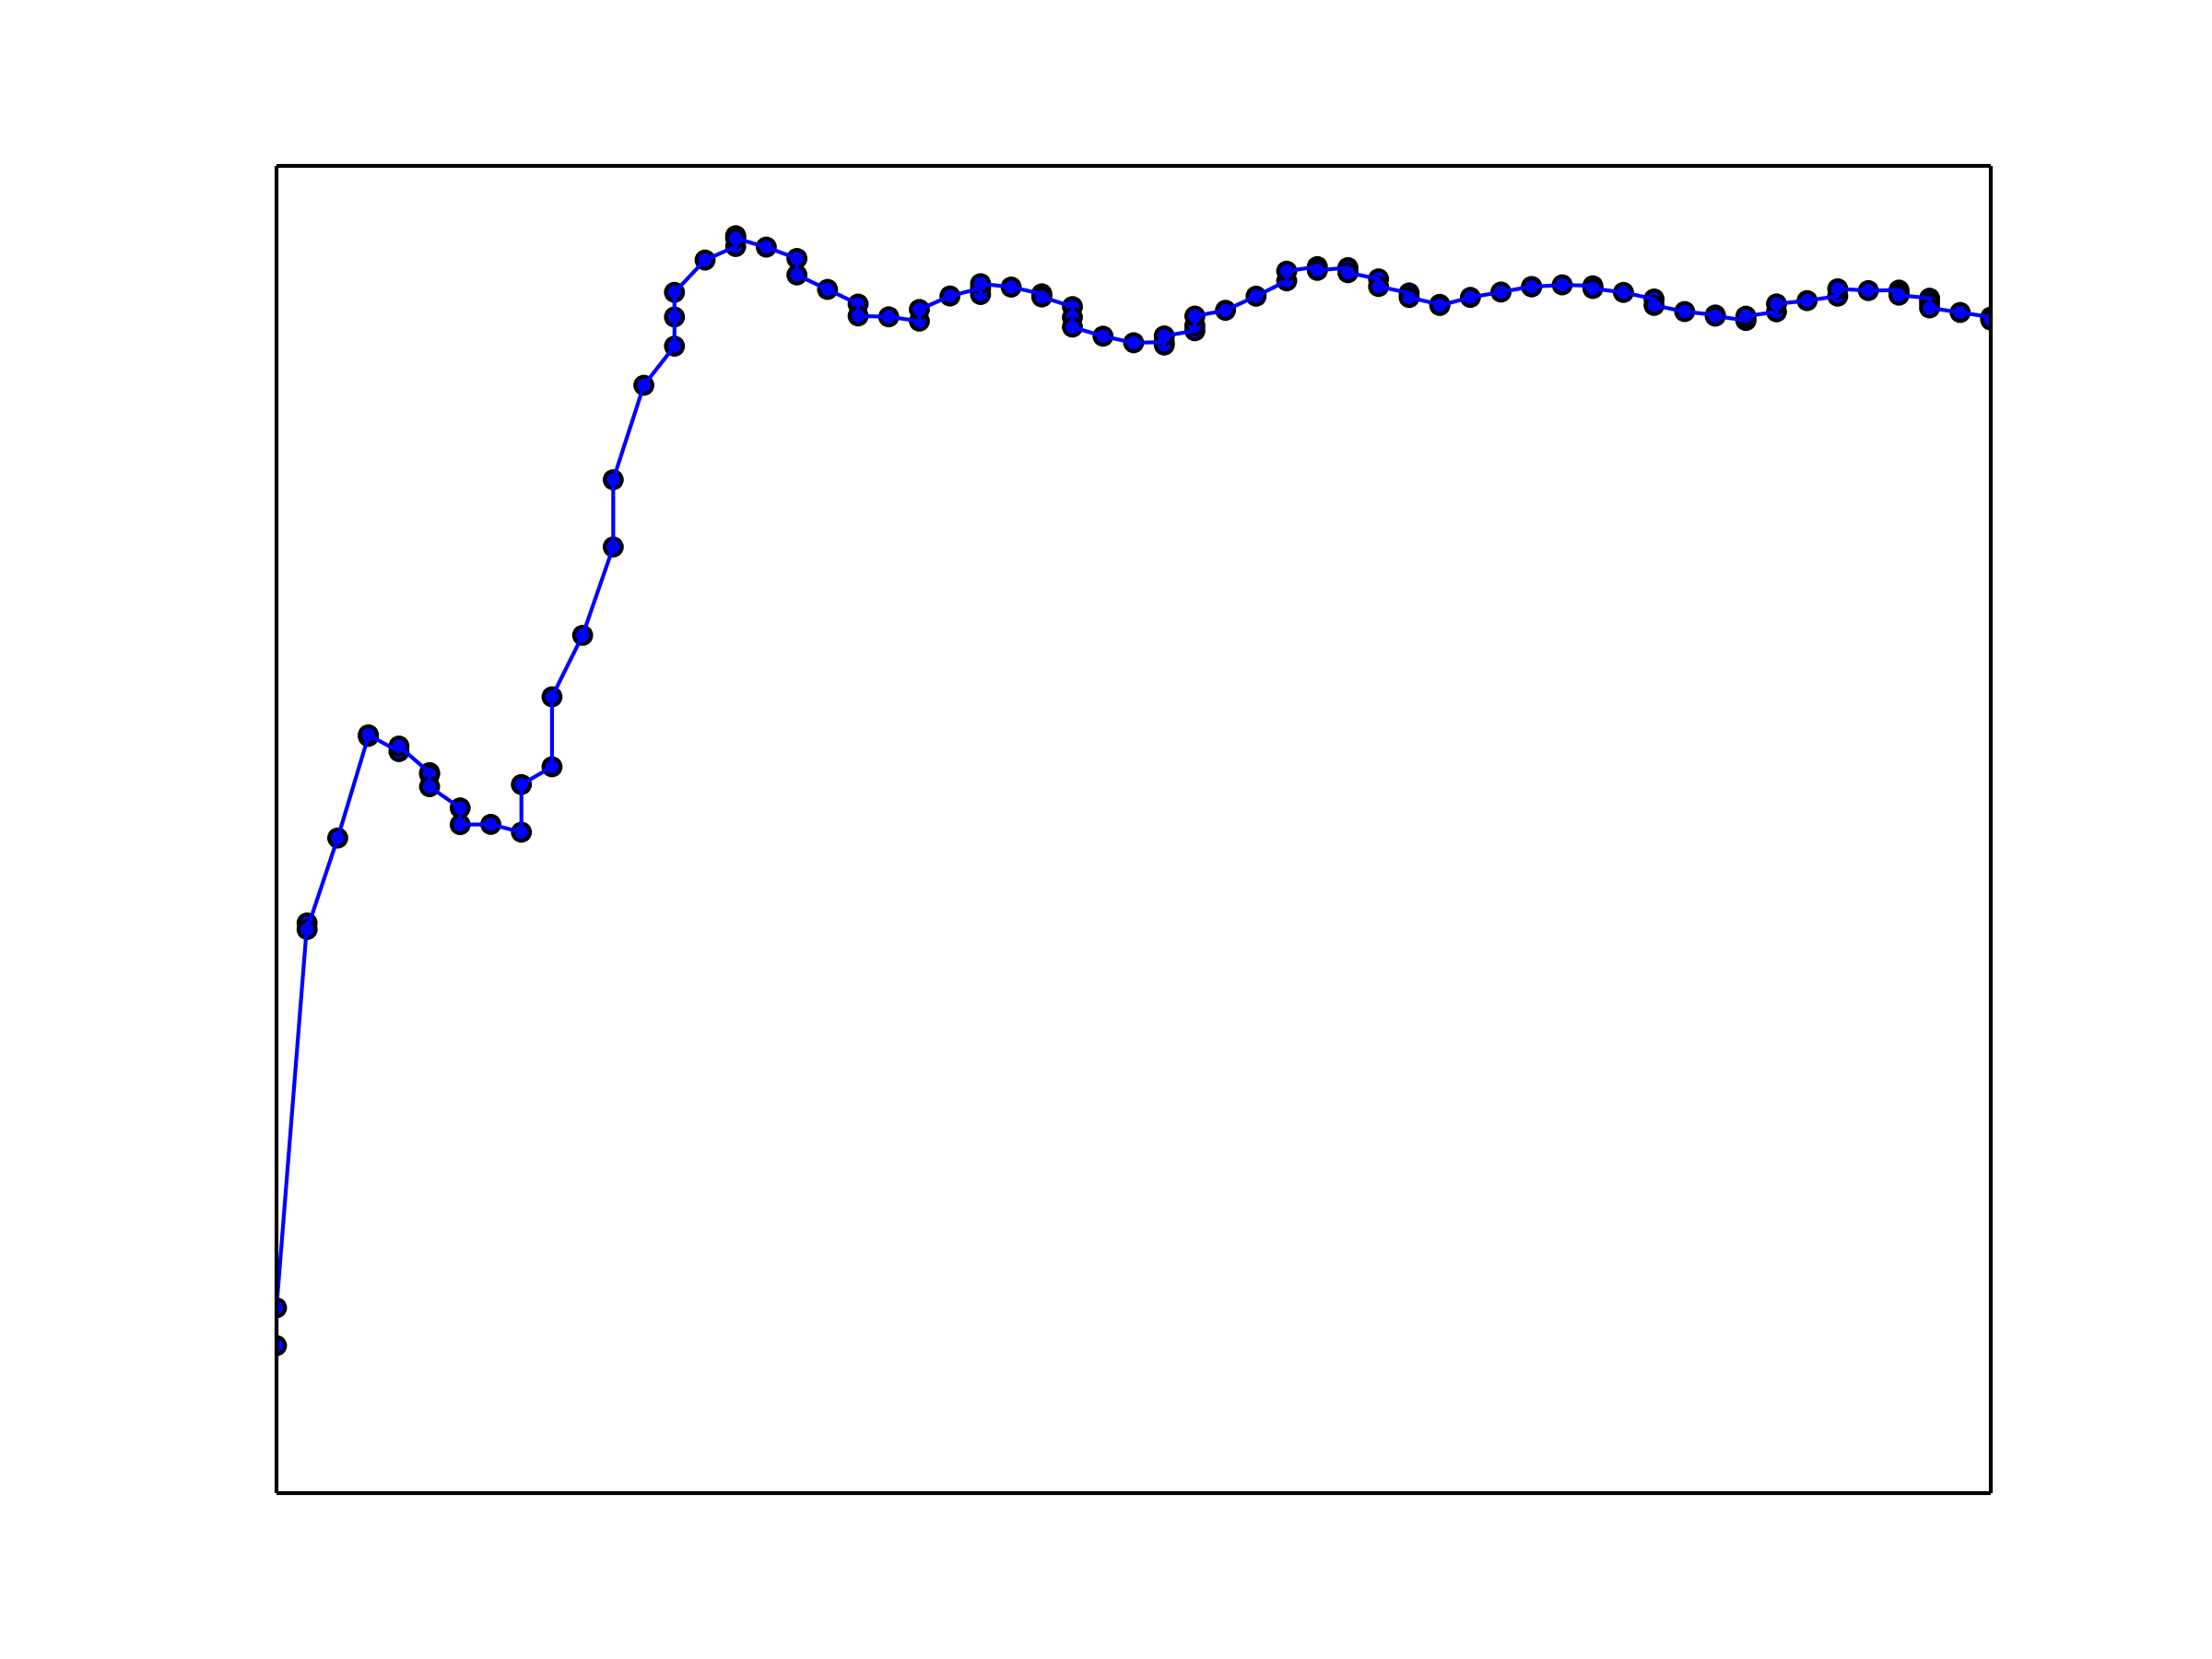
\includegraphics[scale=.5]{./gfx/feature2.png}
    \end{figure}
  \end{frame}

  \begin{frame}[foot]
    \frametitle{\texttt{$1$-lag}}
    \begin{figure}
      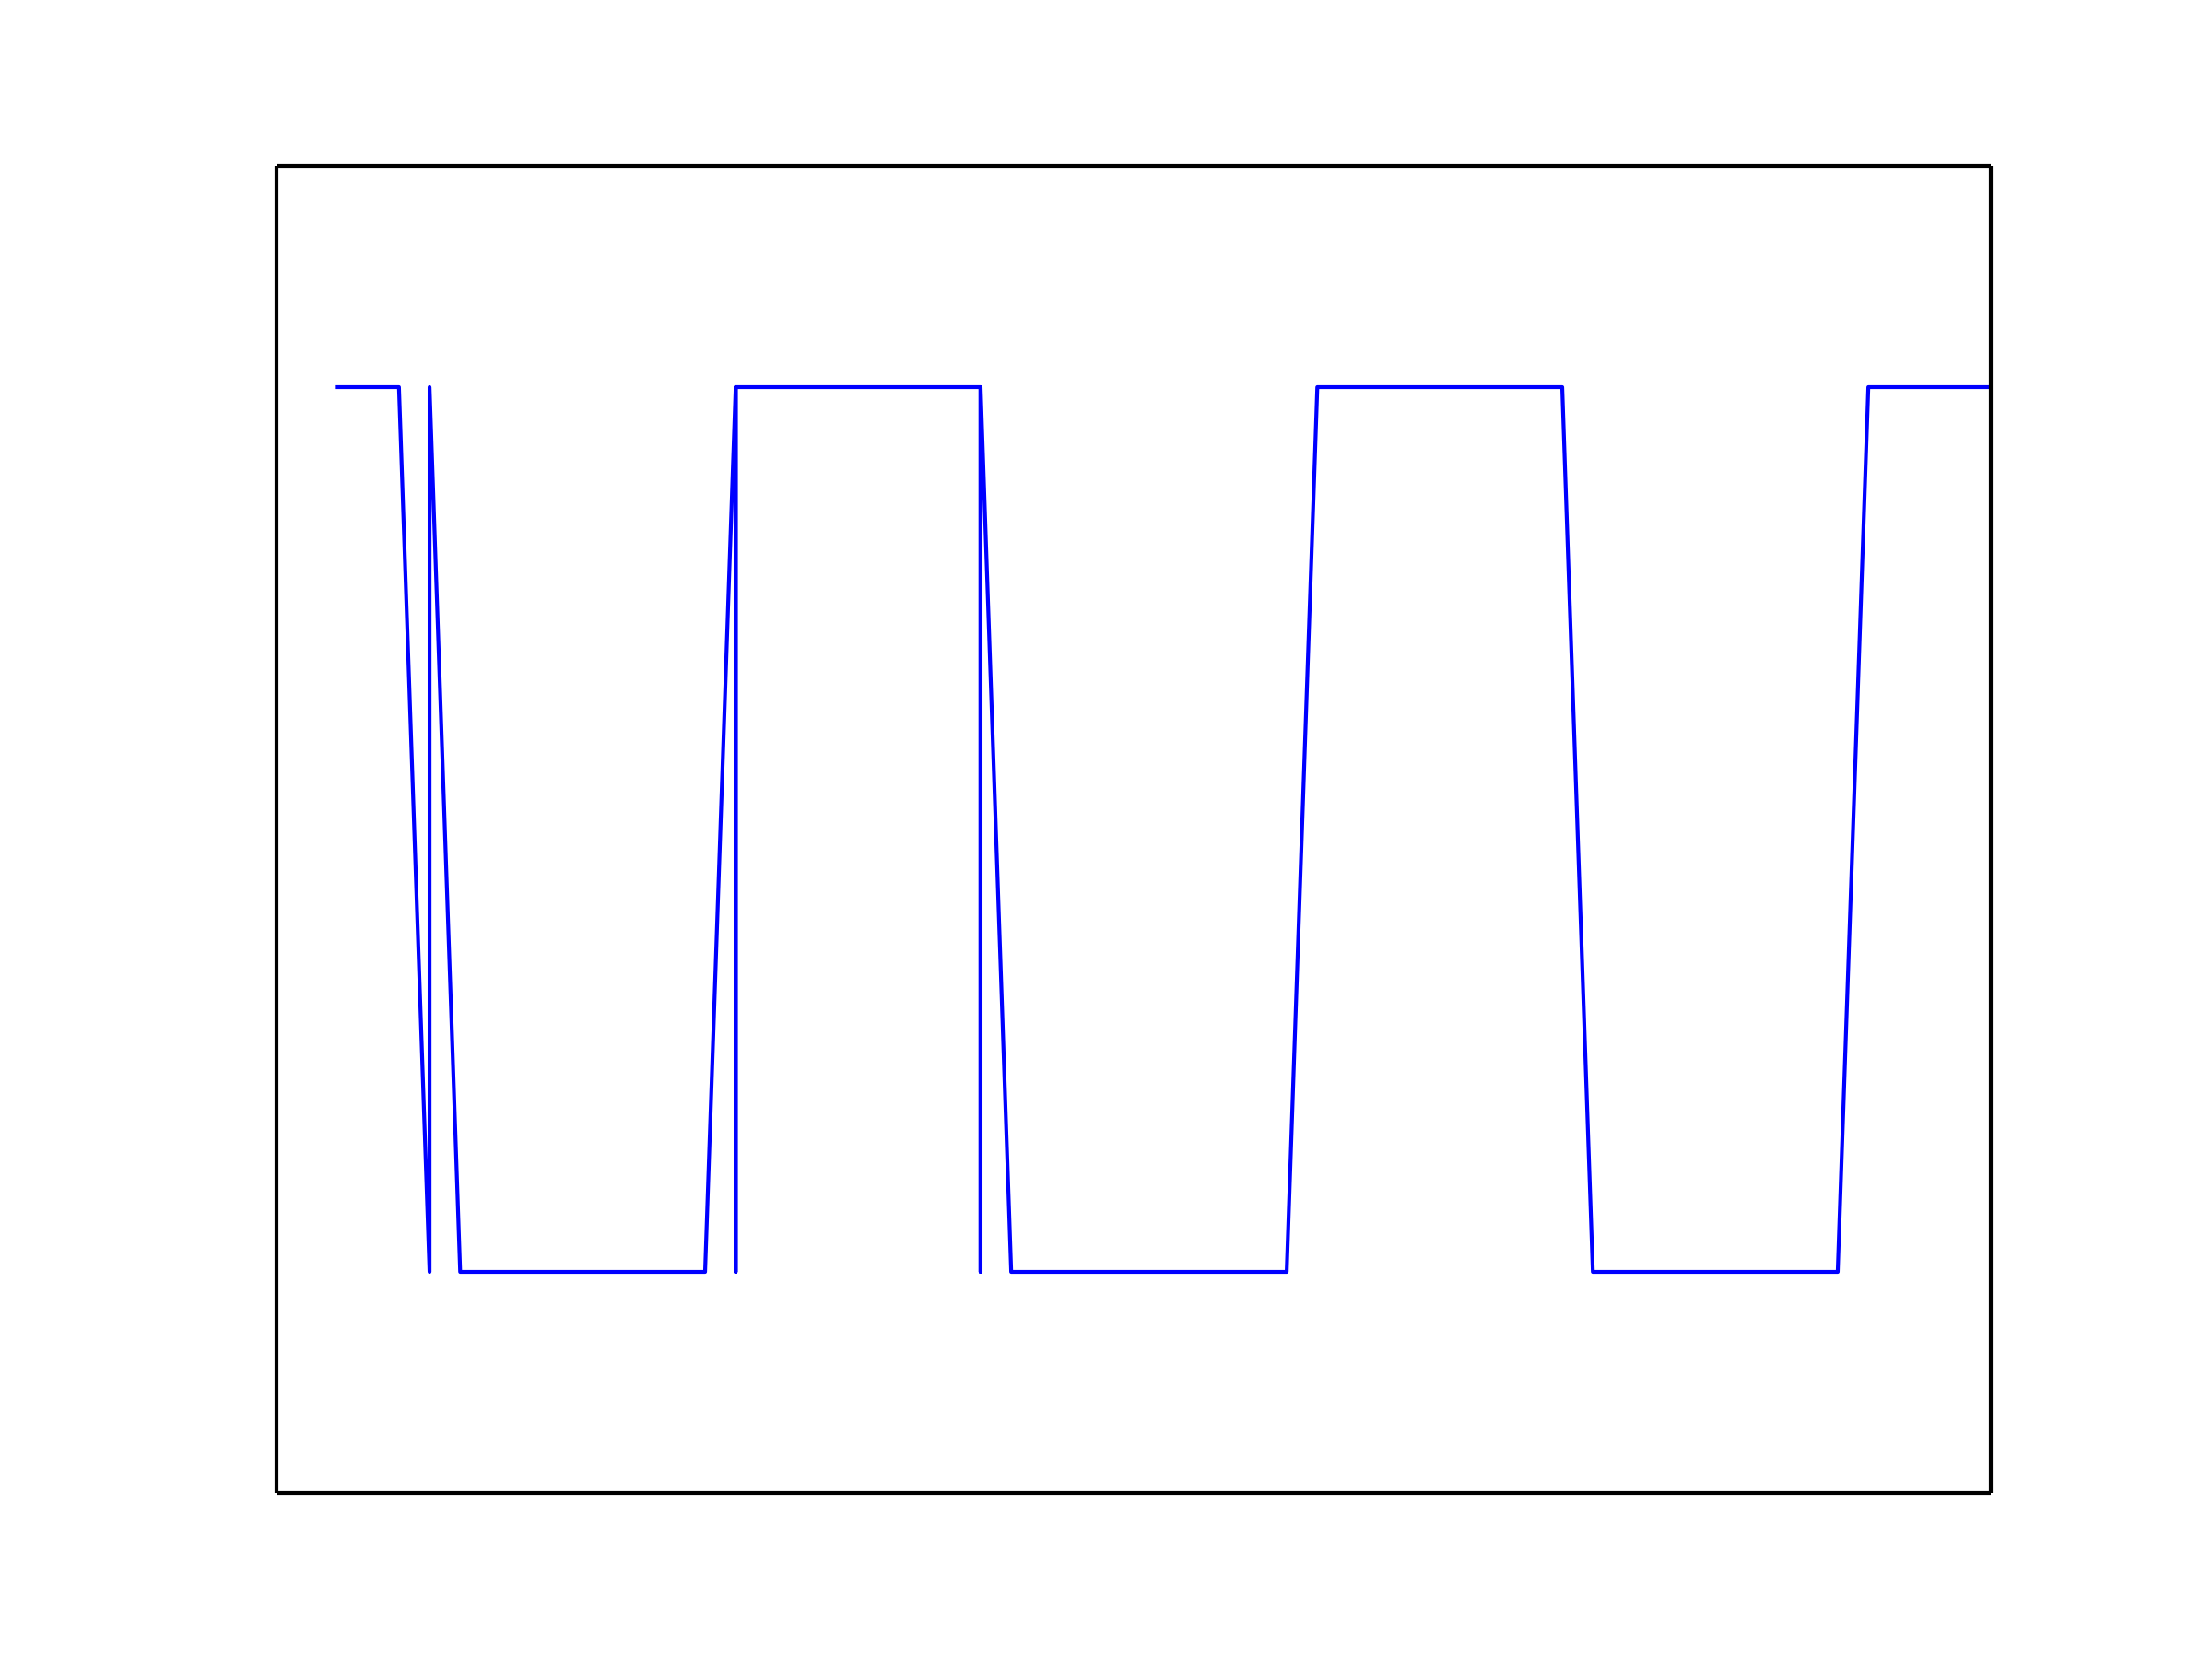
\includegraphics[scale=.5]{./gfx/feature3.png}
    \end{figure}
  \end{frame}

\section{Processing Live Feed}
  % \begin{frame}[foot]
  %   \frametitle{Model of Processing} 
  %   \vspace*{-1.5em}
  %   \begin{figure}[htbp]
  %     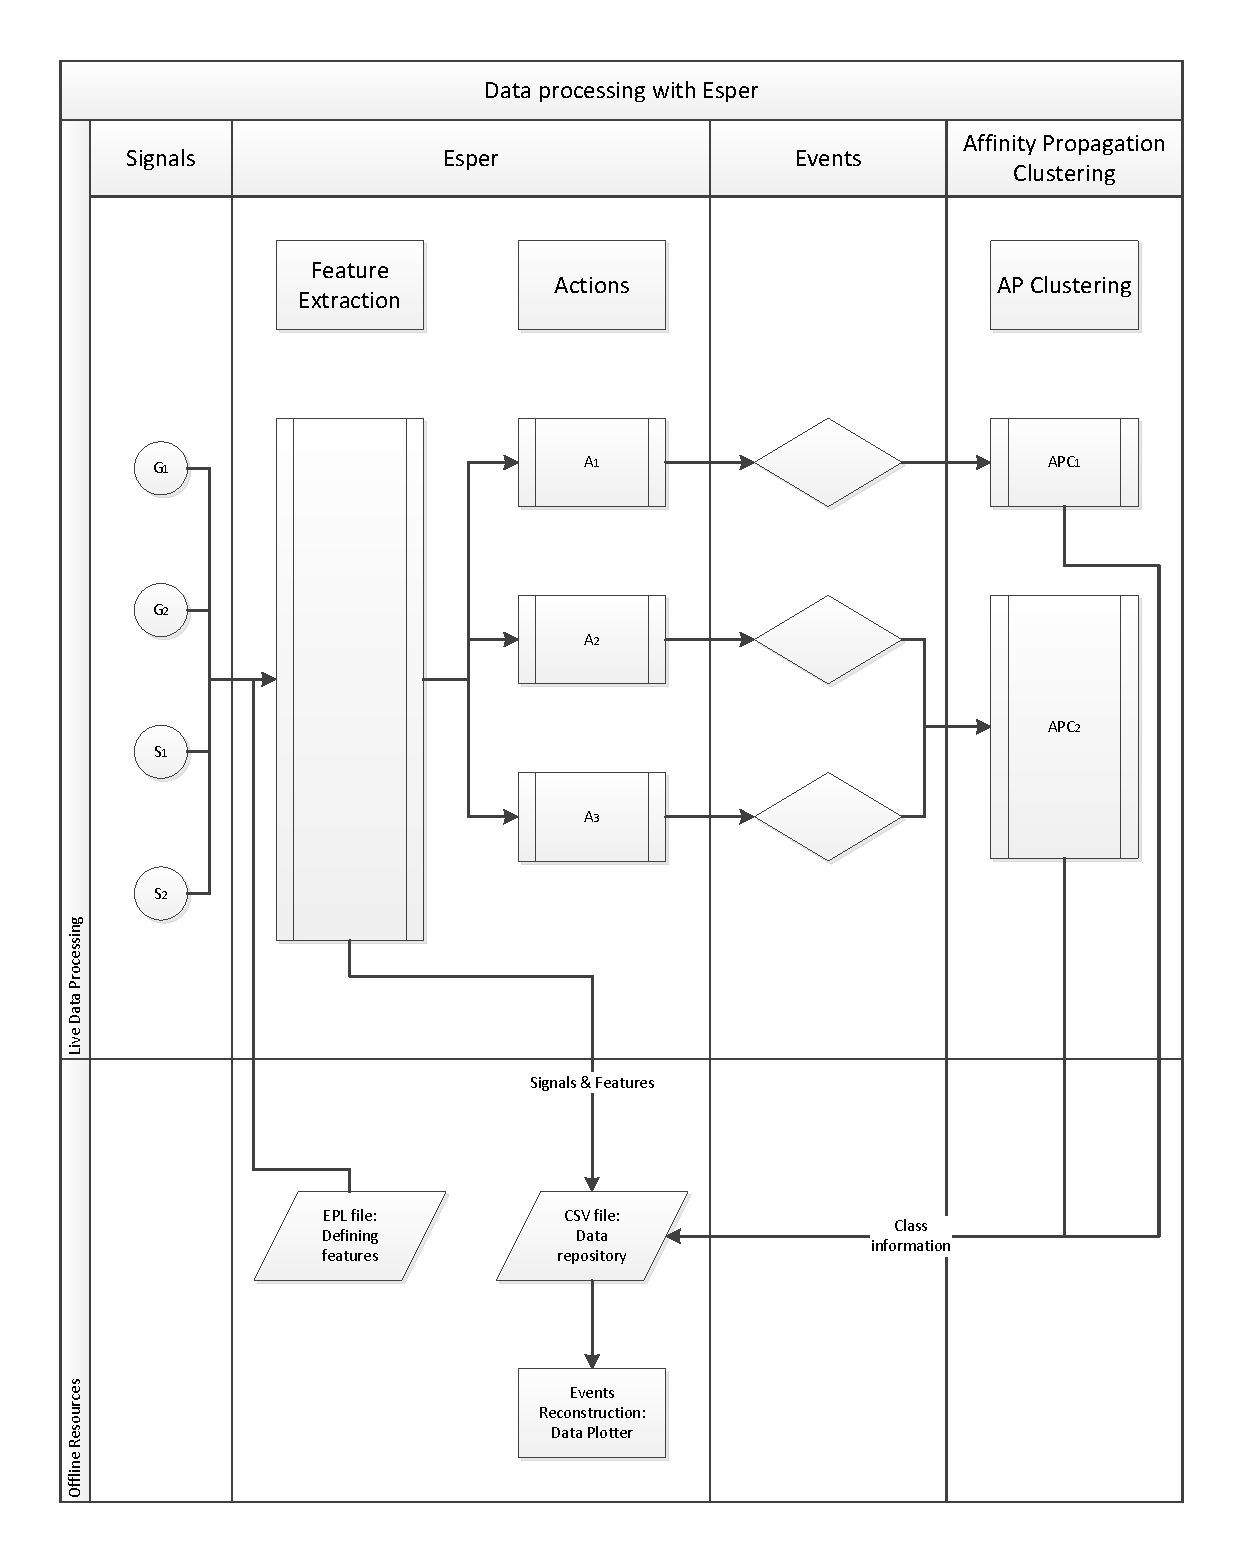
\includegraphics[scale=.4, angle=270]{./gfx/model.pdf}
  %   \end{figure}
  % \end{frame}

  \begin{frame}[containsverbatim, foot]
    \frametitle{Feature Extracting Module}
    \begin{lstlisting}
select
avg(current) as F1,
stddev(current) as F2,
featureExtractors.FeatureExtractor.posNeg
  ( (current - prev(1, current)) ) as F3,
featureExtractors.FeatureExtractor.posNeg
  ( (current - prev(2, current)) ) as F4,
current as F5,
featureExtractors.FeatureExtractor.threshold
  (current) as F6,
6 as FN,
timer as TS
from SinTick.win:time(60 sec);
    \end{lstlisting}
  \end{frame}

  % \section{Clustering}
  % \begin{frame}[foot]
  %   \frametitle{Clustering with \textbf{Affinity Propagation}} 
  %   \begin{block}{Clustering}
  %   ``\\...task of grouping a set of objects in such a way that objects in the same group (called a cluster) are more similar (in some sense or another) to each other than to those in other groups (clusters)...\\''
  %   \end{block}
  %   \pause
  %   \begin{block}{Affinity Propagation}
  %   ``\\...state-of-the-art clustering method recently proposed by Frey and Dueck...based on the concept of "message passing" between data points...unlike (other) clustering algorithms, AP does not require the number of clusters to be determined before running the algorithm...AP finds "exemplars"...\\''
  %   \end{block}
  % \end{frame}

  \begin{frame}[foot]
    \frametitle{Algorithm model} 
    \begin{figure}[htbp]
      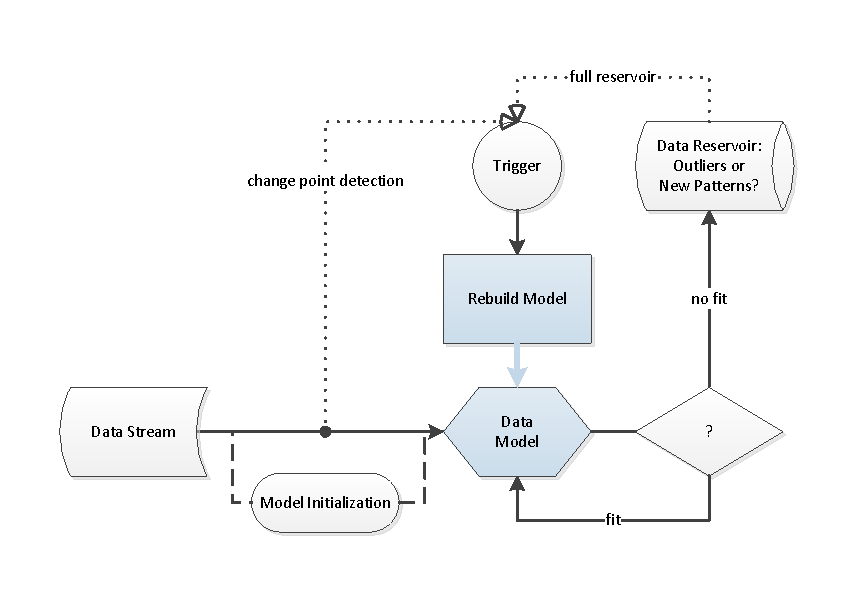
\includegraphics[width=\textwidth]{./gfx/APC.pdf}
    \end{figure}
  \end{frame}

  \begin{frame}[foot]
    \frametitle{Average vs.\ Current} 
    \begin{figure}
      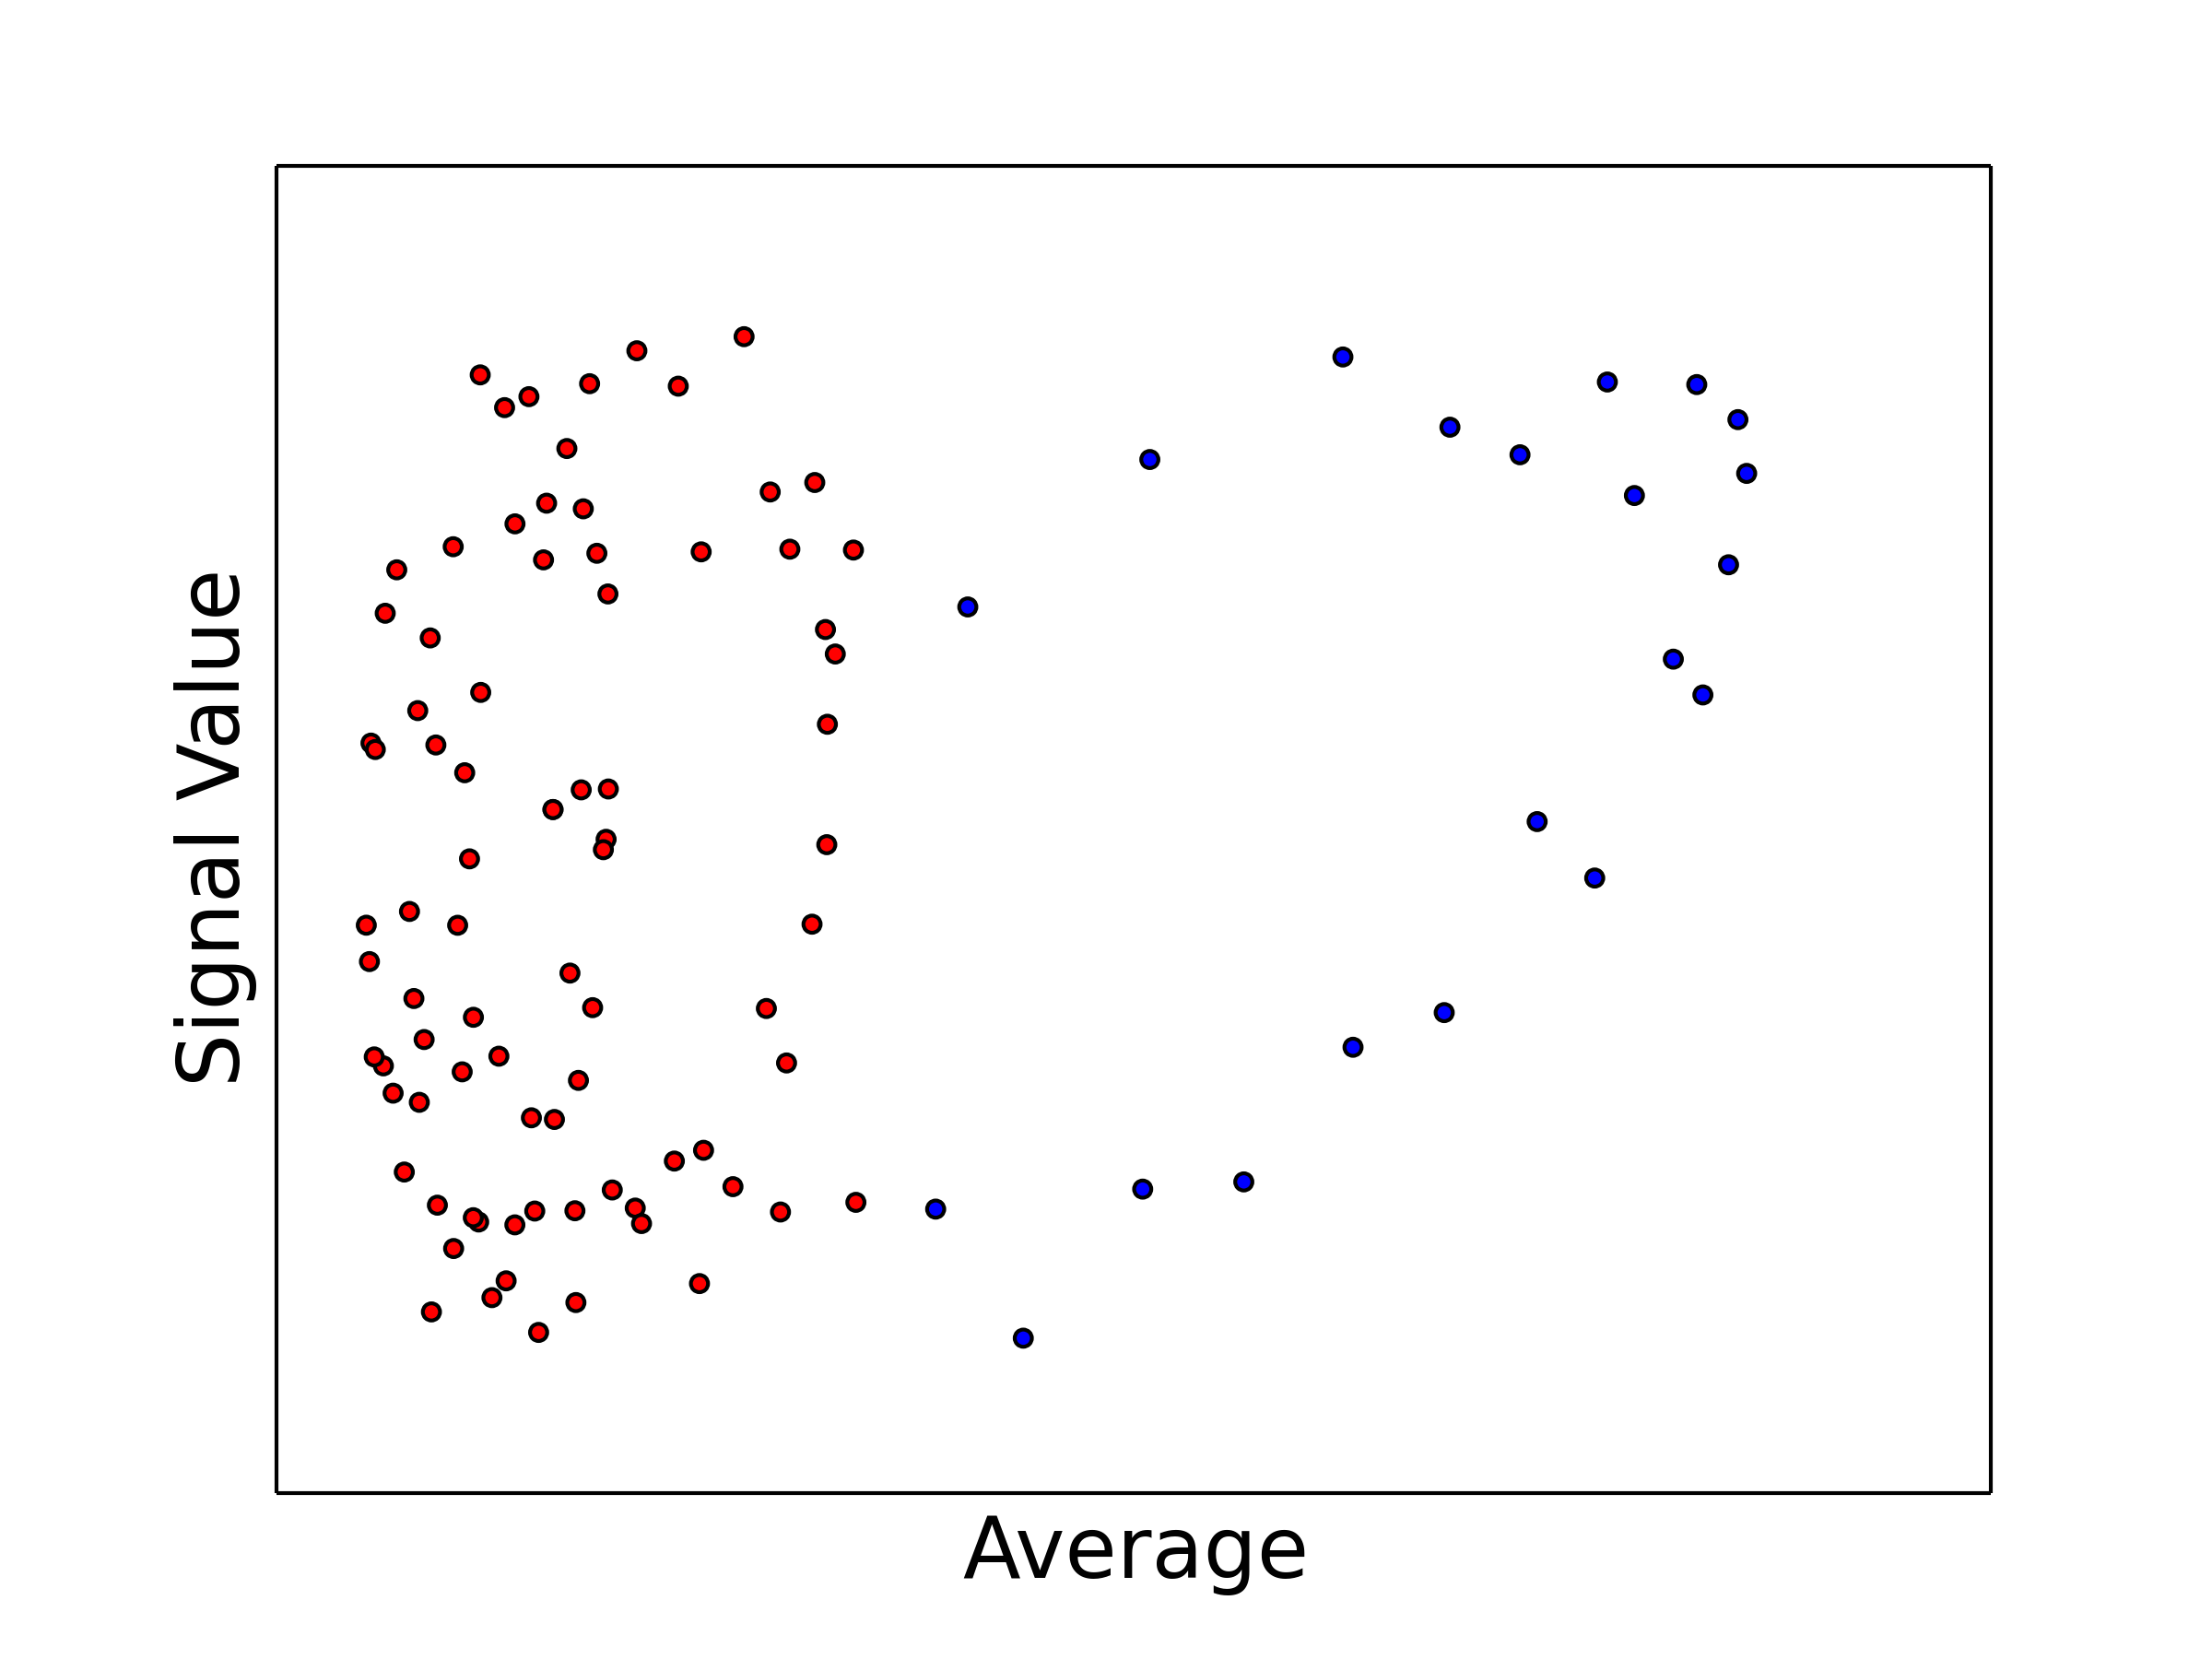
\includegraphics[scale=.5]{./gfx/f1f5.png}
    \end{figure}
  \end{frame}

  \begin{frame}[foot]
    \frametitle{Q\&A}
    \begin{figure}
      
\includegraphics[scale=.5]{./gfx/futurama-fry-meme-00020.jpg}
    \end{figure}
  \end{frame}


% ~\cite{articleExample}
  % \begin{frame}[t, allowframebreaks, plain]
  %   \frametitle{References}
  %   \printbibliography[heading=none]
  % \end{frame}

\end{document}
